%% 
% Preamble
%%
\documentclass[12pt]{article}

\usepackage{hyperref}
\usepackage{setspace}
\usepackage[tocbib,nosectionbib]{apacite}
\usepackage{amsmath}
%\usepackage[nomarkers, figuresonly]{endfloat} % All figures at end of document


\bibliographystyle{apacite}
	\renewcommand{\BOthers}[1]{\emph{et al.}.\hbox{}}
	\renewcommand{\BOthersPeriod}[1]{\emph{et al.}.\hbox{}}

\hypersetup{
	colorlinks = true,
	linkcolor = black,
	urlcolor = blue,
	citecolor = black,
	bookmarks = true}

\doublespacing
\usepackage[pdftex]{graphicx}
\usepackage{keyval}
\begin{document}

\setkeys{Gin}{width=\textwidth, resolution=72}


\renewcommand{\thefigure}{S\arabic{figure}}%
\renewcommand{\thesection}{S\arabic{section}}   
     

%%
% Title page
%%
\begin{titlepage}

\begin{center}

	\textbf{\LARGE Supplementary materials to:}\\
	\vfill
    \textbf{\Large "Quantifying density cues in grouping displays"}\\
    [3em]
    
\onehalfspacing{
    \large    
    Bart Machilsen, Johan Wagemans and Maarten Demeyer\\
    [2em]
    Laboratory of Experimental Psychology\\
    University of Leuven, Belgium\\
    [4em]
    \today
}
\end{center}

\vfill

\begin{flushleft}
\onehalfspacing{
    \textbf{All data and scripts}\\
    \href{https://github.com/mpjdem/densitycue}{https://github.com/mpjdem/densitycue}
}
\end{flushleft}


\begin{flushleft}
\onehalfspacing{
    \textbf{Corresponding author}\\
    Dr. Maarten Demeyer\\
    Tiensestraat 102\\
    3000 Leuven\\
    Belgium\\
    \href{mailto:maarten.demeyer@ppw.kuleuven.be}{maarten.demeyer@ppw.kuleuven.be}\\
    +32 16 326075\\
    [1.5em]
}
\end{flushleft}

\end{titlepage}

\newpage


%%
% Abstract
%%
\section{Performance of other metrics}

In the main text we have compared the performance of five local density metrics in their ability to detect the physical density cue (Section 3.2), to predict the average human performance (Section 3.3), and to select displays without a density cue (Section 3.4). These metrics were the parameter-free \textit{Voronoi} metric, two metrics based on the average distance between neighboring elements (\textit{AvgDist-1} and \textit{AvgDist-3}), and two metrics based on the number of elements within specified radii (\textit{RadCountFull} and \textit{RadCount-2}). These five metrics were the most interesting to compare. Here, we add the results for the eight local density metrics that were not included in the main text: four metrics of the \textit{AvgDist} family (the natural neighbors \textit{AvgDist}, \textit{AvgDist-2}, \textit{AvgDist-4}, and \textit{AvgDist-5}), and four metrics of the \textit{RadCount} family (\textit{RadCount-1.25}, \textit{RadCount-1.5}, \textit{RadCount-1.75}, and \textit{RadCount-2}).

\subsection{Ideal observers: Detection}
\subsubsection{Experiment 1: Contour more dense}

\begin{figure}[h!t]
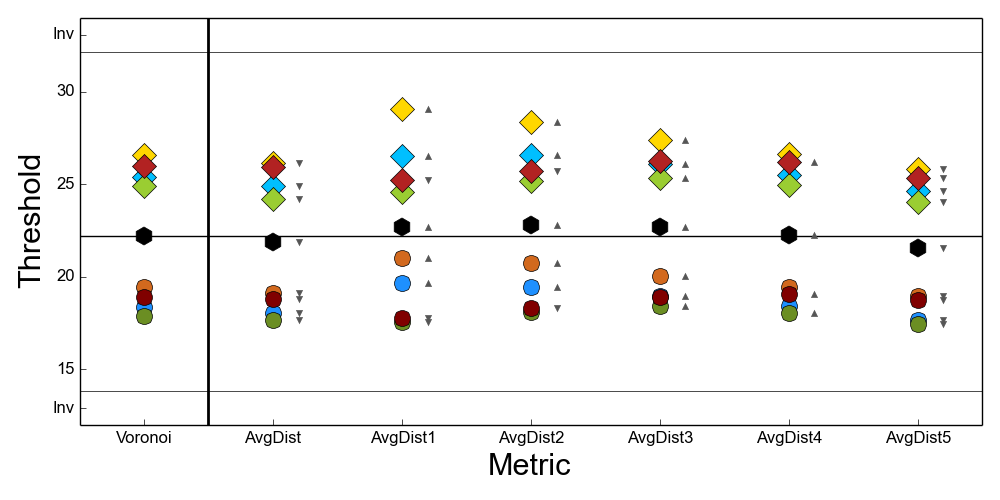
\includegraphics{Figures/FIG_SUP_detect_series_AvgDist_exp1.png}
\caption{Comparison of 75\%-thresholds in Experiment 1 between the \emph{Voronoi} metric and the family of average distance metrics (colors and marker types as in Figure 7 and Figure 9). The \emph{n} following the metric's name corresponds to the number of nearest elements used to calculate the average distance from an element to its neighbors. Black hexagons represent the average threshold across stimulus conditions; significant differences from \emph{Voronoi}, and their  direction, are indicated by triangular markers.}
\label{fig_detect_series_AvgDist_exp1}
\end{figure}

In \autoref{fig_detect_series_AvgDist_exp1} we compare the 75\%-thresholds of the \emph{Voronoi} metric to the 75\%-thresholds of the family of average distance metrics: The parameter-free (natural neighbors) \emph{AvgDist} metric, and five \emph{AvgDist-n} metrics with the number of nearest neighbors, \emph{n}, ranging from 1 to 5. The parameter-free \emph{AvgDist} metric performs slightly worse than the \emph{Voronoi} metric. \emph{AvgDist-1} - which only takes into account the single nearest neighbor - performs better on the Random conditions, but tends to be worse at the Equidistant conditions. The same holds to a lesser extent for the \emph{AvgDist-2} metric. \emph{AvgDist-3} is a better cue detector than \emph{Voronoi} in all conditions, whereas \emph{AvgDist-4} is comparable to \emph{Voronoi}, and \emph{AvgDist-5} performs worse.\\

\autoref{fig_detect_series_RadCount_exp1} illustrates a similar comparison between the \emph{Voronoi} metric and the family of radius count metrics: The parameter-free (range of radii) \emph{RadCountFull} metric, and five \emph{RadCount-r} metrics with a fixed radius \emph{r} ranging from 1.25 to 2.25 times the minimum distance between background elements. For \emph{RadCountFull}, this is the case for all Equidistant stimulus categories, indicating high detection performance regardless of contour spacing. In other words, this metric detects the regularity of contour spacings in these displays. There is also an advantage present in the Random conditions, where performance is better than \emph{Voronoi}. The lower two fixed-radius \emph{RadCount} metrics display bad fits, and are not usable in practice. Of the higher three of these metrics, \emph{RadCount-2} is closest to \emph{Voronoi}, although significantly worse.

\begin{figure}[h!t]
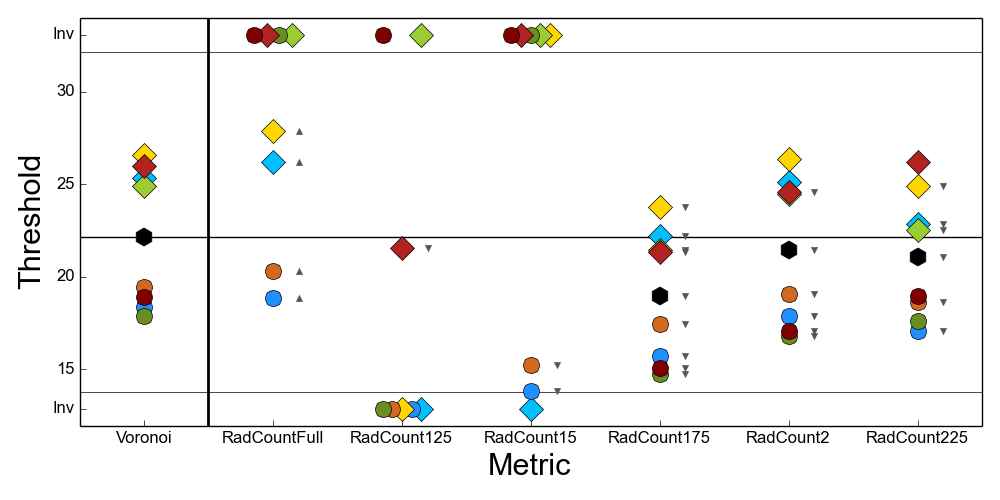
\includegraphics{Figures/FIG_SUP_detect_series_RadCount_exp1.png}
\caption{Comparison of 75\%-thresholds in Experiment 1 between the \emph{Voronoi} metric and the family of radius count metrics (colors and marker types as in Figure 10 and Figure 12). The number in the metric's name corresponds to the radius parameter used, in units of minimum distance between background elements. Black markers represent the average threshold across stimulus conditions; significant differences from \emph{Voronoi}, and their direction, are indicated by triangular markers. The Inv (invalid) categories hold data points where the 75\%-thresholds exceed the data range.}
\label{fig_detect_series_RadCount_exp1}
\end{figure}

\subsubsection{Experiment 2: Contour more sparse}

\begin{figure}[h!t]
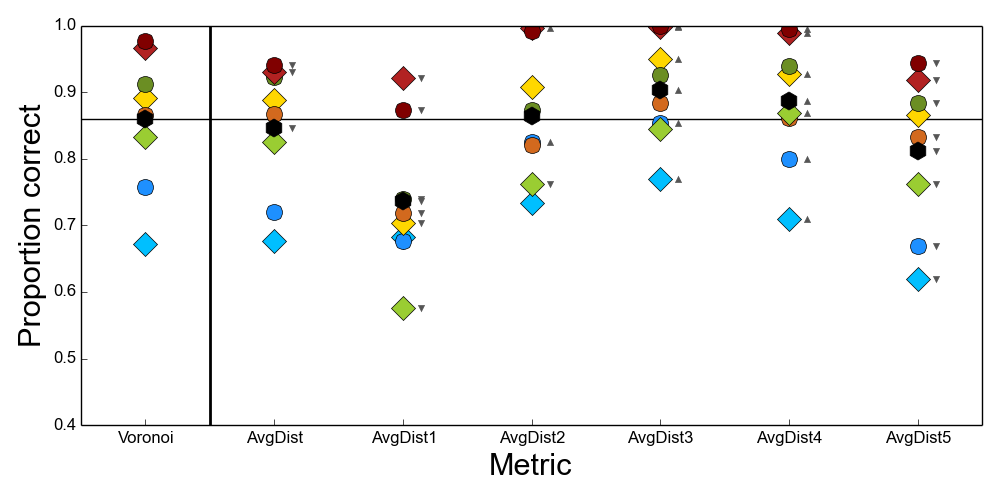
\includegraphics{Figures/FIG_SUP_detect_series_AvgDist_exp2.png}
\caption{Comparison of performances in Experiment 2 between the \emph{Voronoi} metric and the family of average distance metrics. Marker types correspond to Figure 10 and Figure 12.}
\label{fig_detect_series_AvgDist_exp2}
\end{figure}

\autoref{fig_detect_series_AvgDist_exp2} and \autoref{fig_detect_series_RadCount_exp2} plot the ideal observer performances for Experiment 2, in its single contour spacing condition. It can be seen that whereas humans were unable to do this task, the ideal observers perform well. This is especially the case for the \emph{Voronoi} metric, the family of \emph{AvgDist} metrics (especially \emph{AvgDist-3}), and the \emph{RadCountFull} metric. The fixed-radius \emph{RadCount} metrics perform worse, with the exception of \emph{RadCount-1.25}. It remains to be seen, however, whether this very specific benefit would still hold across a larger range of sparse contour spacing levels. In general, the Open contours are less easily detected, especially in conditions with Random element placement.

\begin{figure}[h!t]
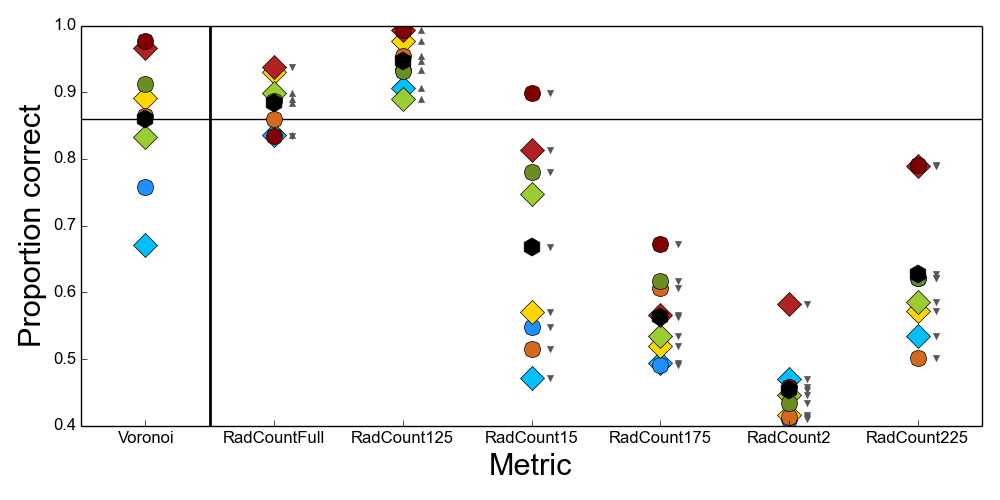
\includegraphics{Figures/FIG_SUP_detect_series_RadCount_exp2.png}
\caption{Comparison of performances in Experiment 2 between the \emph{Voronoi} metric and the family of radius count metrics. Marker types correspond to Figure 10 and Figure 12.}
\label{fig_detect_series_RadCount_exp2}
\end{figure}


\subsection{Ideal observers: Prediction}

In this section we quantify each metric's ability to predict the 64 condition means of Experiment 1, and statistically compare it to the predictive validity of the \textit{Voronoi} metric. \autoref{fig_predict_series_AvgDist_exp1} shows this comparison for the family of \textit{AvgDist} metrics. Of these metrics, only the parameter-free \textit{AvgDist} metric and \textit{AvgDist-5} are better at predicting mean human performance than the \textit{Voronoi} metric, both in terms of explained variability within stimulus conditions (higher red bars in \autoref{fig_predict_series_AvgDist_exp1}) and in terms of consistency across stimulus conditions (lower green bars in \autoref{fig_predict_series_AvgDist_exp1}).\\

\begin{figure}
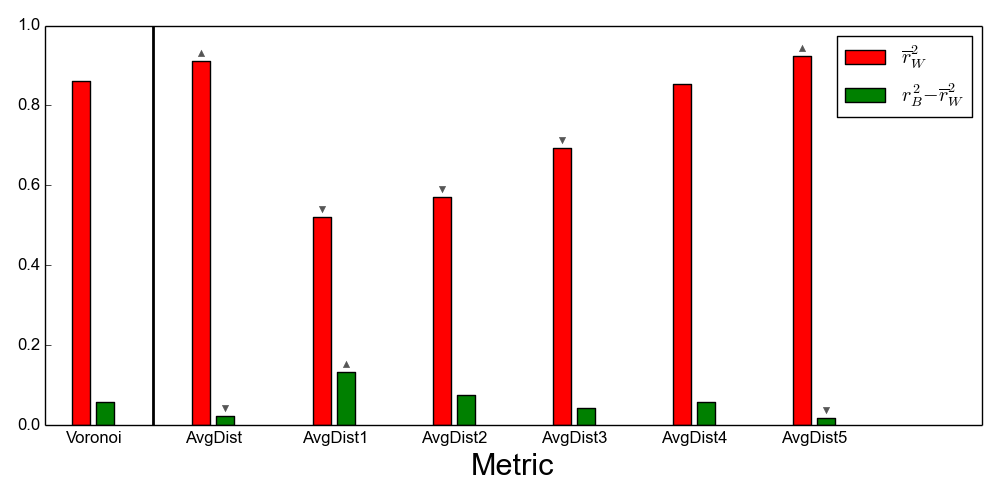
\includegraphics{Figures/FIG_SUP_predict_series_AvgDist_exp1.png}
\caption{Comparison of predictive validity between the \emph{Voronoi} metric and the family of average distance metrics: The parameter-free (natural neighbors) \emph{AvgDist} metric and the five fixed-parameter \emph{AvgDist-n} metrics. $\overline{r}^{2}_W$ is the within-condition coefficient of determination, averaged across conditions; $r^{2}_B$ is the coefficient of determination across all eight stimulus conditions. High values of $\overline{r}^{2}_W$ (red bars) indicate strong within-condition correspondence between a metric and the human data. Low values of $r^{2}_B -\overline{r}^{2}_W$ (green bars) indicate a high consistency across stimulus conditions. Statistical significance is indicated through the triangular markers.}
\label{fig_predict_series_AvgDist_exp1}
\end{figure}

A similar comparison is made for the family of radius count metrics in \autoref{fig_predict_series_RadCount_exp1}. No member of the radius count family has better predictive validity of the condition means than the \emph{Voronoi} metric. Only \emph{RadCount-2} is statistically similar to \emph{Voronoi} in predicting human performance within and across stimulus conditions.

\begin{figure}
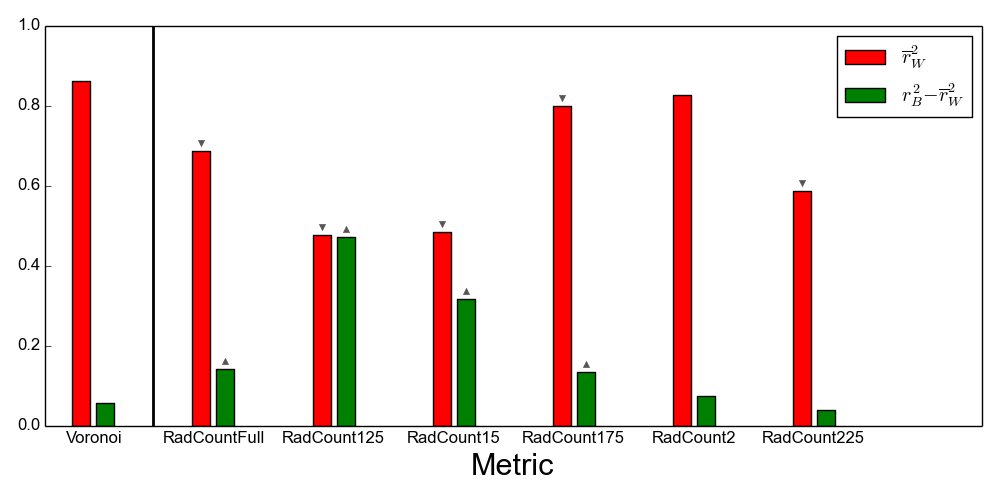
\includegraphics{Figures/FIG_SUP_predict_series_RadCount_exp1.png}
\caption{Comparison of predictive validity between the \emph{Voronoi} metric and the family of radius count metrics: The parameter-free \emph{RadCountFull} metric and the five fixed-parameter \emph{RadCount-r} metrics.}
\label{fig_predict_series_RadCount_exp1}
\end{figure}



\subsection{Ideal observers: Selection}

\subsubsection{Absence of local density cues}

We now evaluate which metrics offer suitable criteria for the selection of stimuli in which human observers cannot detect the target contour. For this purpose, we analyze human performance on a subset of trials where the metric did not detect a local density difference, i.c. trials with a value \emph{p} between 0.35 and 0.65 (the selected trials differ between metrics).

\begin{figure}
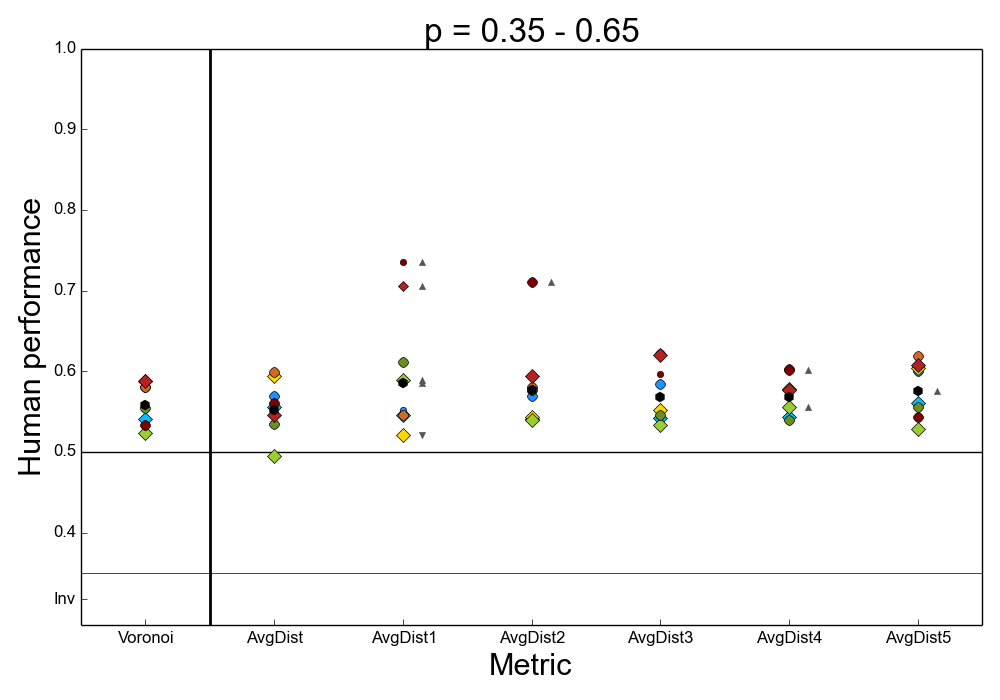
\includegraphics{Figures/FIG_SUP_select_series_AvgDist_exp1_3565.png}
\caption{Average human performance on a subset of trials for which the \emph{AvgDist} metric of interest returned a \emph{p} between 0.35 and 0.65 (i.e., almost complete absence of density cue, according to the metric). The marker size is proportional to the number of retained stimuli.}
\label{fig_select_series_AvgDist_exp1_3565}
\end{figure}


\autoref{fig_select_series_AvgDist_exp1_3565} plots the average human performance for trials with $0.35 < p < 0.65$ on a given metric of the \textit{AvgDist} family. All metrics provide reasonable selection criteria, as evidenced by an average human performance (black markers) below 60\% correct on the retained trials. For these trials, the metric of interest found (almost) no evidence for the presence of a local density cue. No metric performs significantly better than \emph{Voronoi}. The \emph{AvgDist} metric computed from the distance to the natural neighbors is at the same level as the \emph{Voronoi} metric, as are \emph{AvgDist-2}, \emph{AvgDist-3}, and \emph{AvgDist-4}. The \emph{AvgDist-1} and \emph{AvgDist-5} metrics perform significantly worse than \emph{Voronoi}. Interestingly, the \textit{AvgDist-1} metric computed from the distance to the nearest neighbor is excellent at selecting the Random display types, but not good at selecting the Equidistant displays. The \emph{Voronoi} metric seems to be the most stable across stimulus conditions.

\begin{figure}
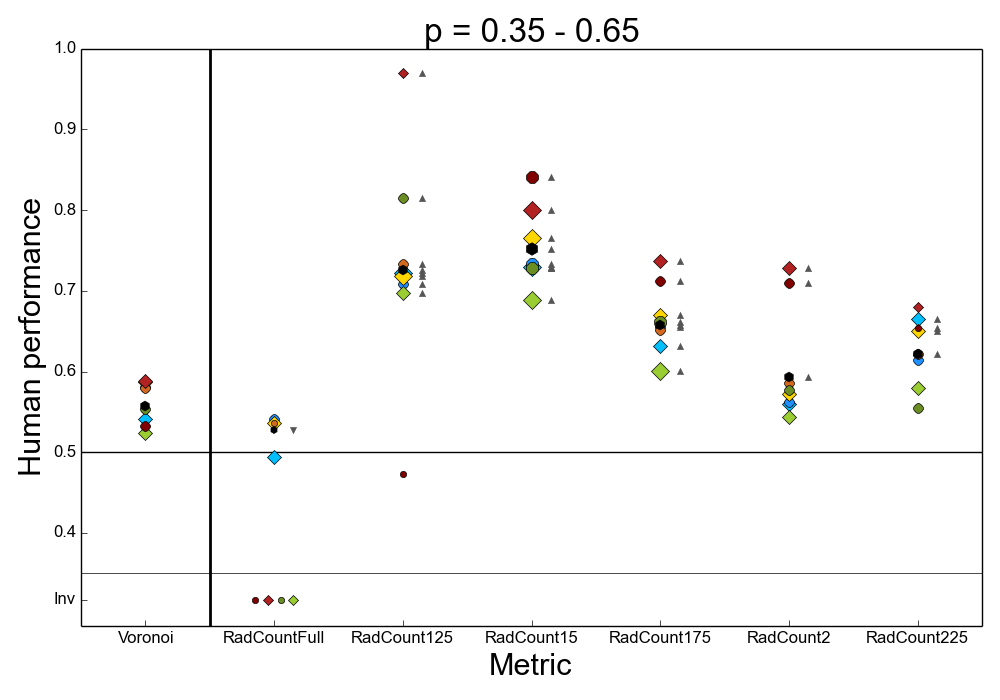
\includegraphics{Figures/FIG_SUP_select_series_RadCount_exp1_3565.png}
\caption{Average human performance on a subset of trials for which the \emph{RadCount} metric of interest returned a \emph{p} between 0.35 and 0.65 (i.e., almost complete absence of density cue, according to the metric). The marker size is proportional to the number of retained stimuli.}
\label{fig_select_series_RadCount_exp1_3565}
\end{figure}

The comparison between the \emph{RadCount} family of metrics and \emph{Voronoi} is presented in \autoref{fig_select_series_RadCount_exp1_3565}. Except for \emph{RadCountFull}, all metrics perform significantly worse than \emph{Voronoi}, with selection performance depending strongly on the exact value of the spacing parameter. The \emph{RadCountFull} metric seems to be very sensitive to the regularity in spacing along the contour, retaining almost no trials in the Equidistant stimulus conditions.

\subsubsection{Contour more sparse than background}

Here we again compare the \emph{Voronoi} metric on the one hand, and the family of \emph{AvgDist} and \emph{RadCount} metrics on the other hand, but now for the selection bin $0.65 < p < 1$. For the displays in this bin the density along the contour is significantly lower than the density in the background.

\begin{figure}
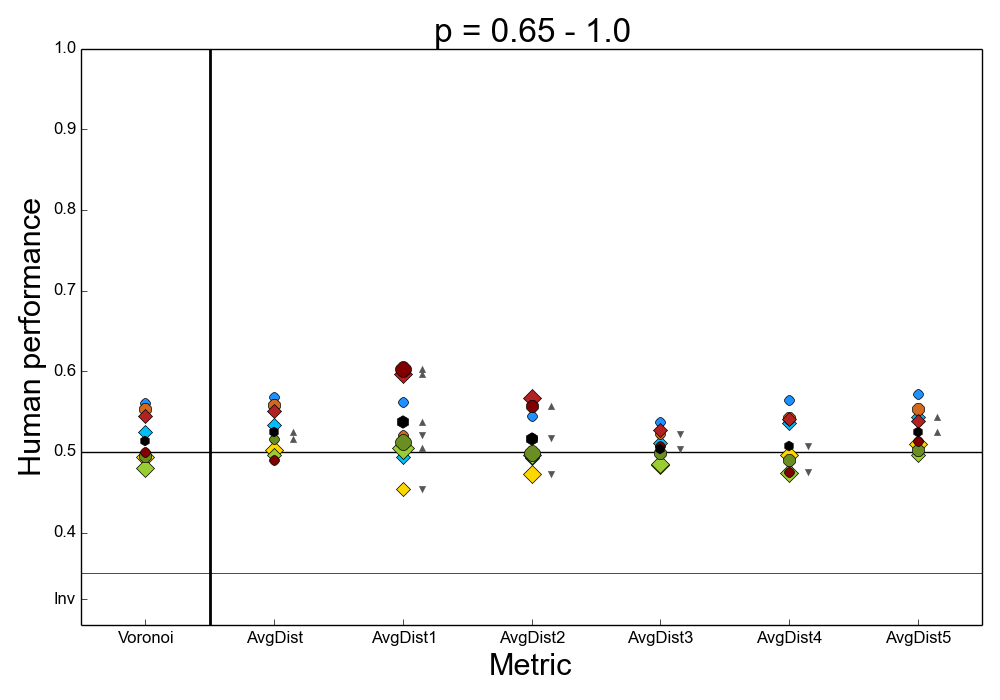
\includegraphics{Figures/FIG_SUP_select_series_AvgDist_exp1_651.png}
\caption{Average human performance on a subset of trials for which the \emph{AvgDist} metric of interest returned a \emph{p} between 0.65 and 1.0 (i.e., contour more sparse than background, according to the metric).}
\label{fig_select_series_AvgDist_exp1_651}
\end{figure}

\autoref{fig_select_series_AvgDist_exp1_651} plots this comparison for the family of \textit{AvgDist} metrics. The natural neighbors \emph{AvgDist} metric, \emph{AvgDist-1}, and \emph{AvgDist-5} perform significantly worse than the \emph{Voronoi} metric. The metrics that compute the distance to the 2, 3, and 4 nearest neighbors are significantly better. For the \emph{AvgDist-3} metric human performance is at chance level (50.3\%, z=0.6).

In \autoref{fig_select_series_RadCount_exp1_651} we compare the \emph{Voronoi} metric to the family of \emph{RadCount} metrics for the same selection bin. Compared to the \emph{Voronoi} metric, all \emph{RadCount} metrics perform significantly worse and are more variable between conditions. Again, the performance depends strongly on the exact value of the spacing parameter.

\begin{figure}
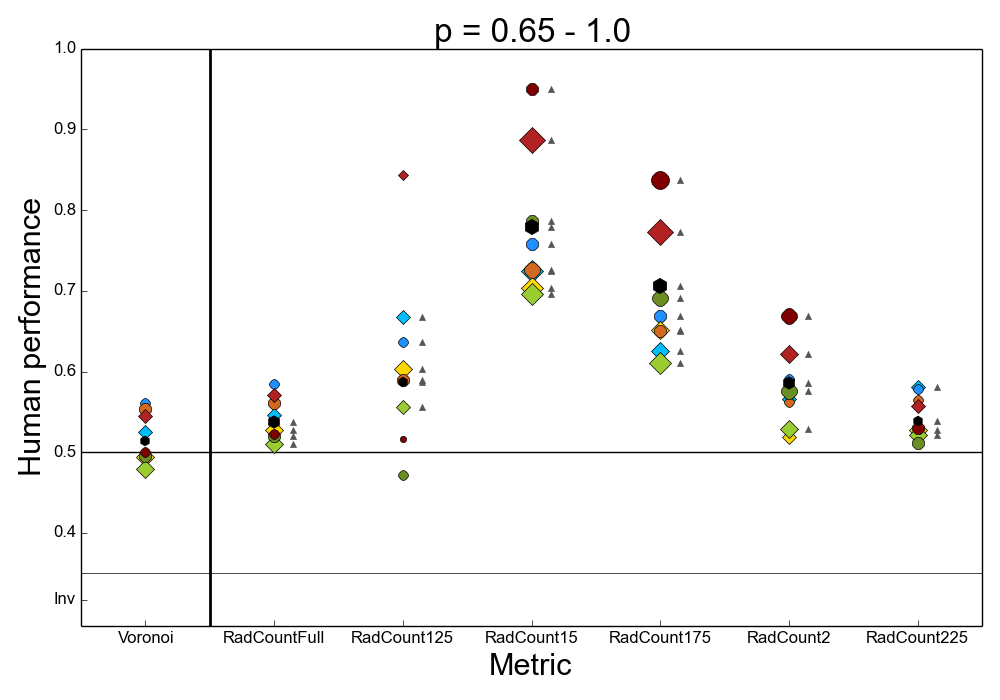
\includegraphics{Figures/FIG_SUP_select_series_RadCount_exp1_651.png}
\caption{Average human performance on a subset of trials for which the \emph{RadCount} metric of interest returned a \emph{p} between 0.65 and 1.0 (i.e., contour more sparse than background, according to the metric).}
\label{fig_select_series_RadCount_exp1_651}
\end{figure}

%%
% D
%%
\section{Comparison with D}
\label{section_comparison_D}
In the literature on contour integration, Kov{\'a}cs and colleagues have introduced a density measure D (also referred to as \emph{delta}, \emph{relative noise density}, or \emph{signal-to-noise ratio}) that expresses the ratio of background spacing to contour spacing. They have used D to measure the strength of contour integration in individual observers: The lower the value of D at detection threshold, the stronger the contour integration \cite<e.g.,>{Kovacs00}. In the stimulus construction process, D is used as a parameter to manipulate the salience of the embedded contour. It is claimed that when $D>1$, the contour can be detected from the difference in element spacing between contour and background. When $D\leq1$, however, this cue is not present and additional orientation cues are needed to detect the contour \cite<e.g.,>{Kovacs99}. At first sight, the measure D is similar to the criterion p that we have introduced in the GERT toolbox \cite{Demeyer12}. Indeed, when evaluated on all trials of our Experiment 1, D and p are strongly correlated (r=-0.71). However, D and p also differ in several respects. Here we will describe the key differences between D and our measure p.\\

From what we have gathered from published method sections \cite{Kovacs99,KovacsPolat00,Silverstein00,Silverstein09}, D expresses the ratio of the average Euclidean distance of each background element to adjacent elements (essentially, the AvgDist metric of the current manuscript), to the average Euclidean distance between neighboring contour elements. Note that this implies a different method of density quantification for contour and background elements. For contour spacing, the distance between its ordered contour elements is calculated, whereas background spacing is computed on unordered elements. Moreover, in computing only a single density estimate for both contour and background, abstraction is made of both density variations within the display, and the relative number of contour versus background elements. The definition of D implies that it can only be a global measure of the density differences in a display, whereas the GERT methods are based on truly local density estimates - for each element individually in the same manner, regardless of whether they are contour or background elements. Then, the difference between the average contour density and the average background density is expressed in relation to the local density variation within the display, as p. p constitutes a common scale on which different metrics can be compared, and a meaningful if arbitrary selection criterion can be set.\\

A consequence of D's global nature is that it can unfortunately not be evaluated using the same analyses as were performed in the current manuscript, which necessitate truly local density estimates for each element. However, in \autoref{fig_D}, we do plot simply the dependence of human performance on D in our own data. It can be seen that as expected, a strong monotonous relationship is present for all conditions. There is, however, also a strong separation of the curves between conditions - the D value is not the sole determinant of human performance. Most importantly however, using a criterion of $D<1$ is indeed a valid method to ensure near-chance human performance in any condition, with the highest condition performances around 55\% correct at $D=1$.\\

\begin{figure}
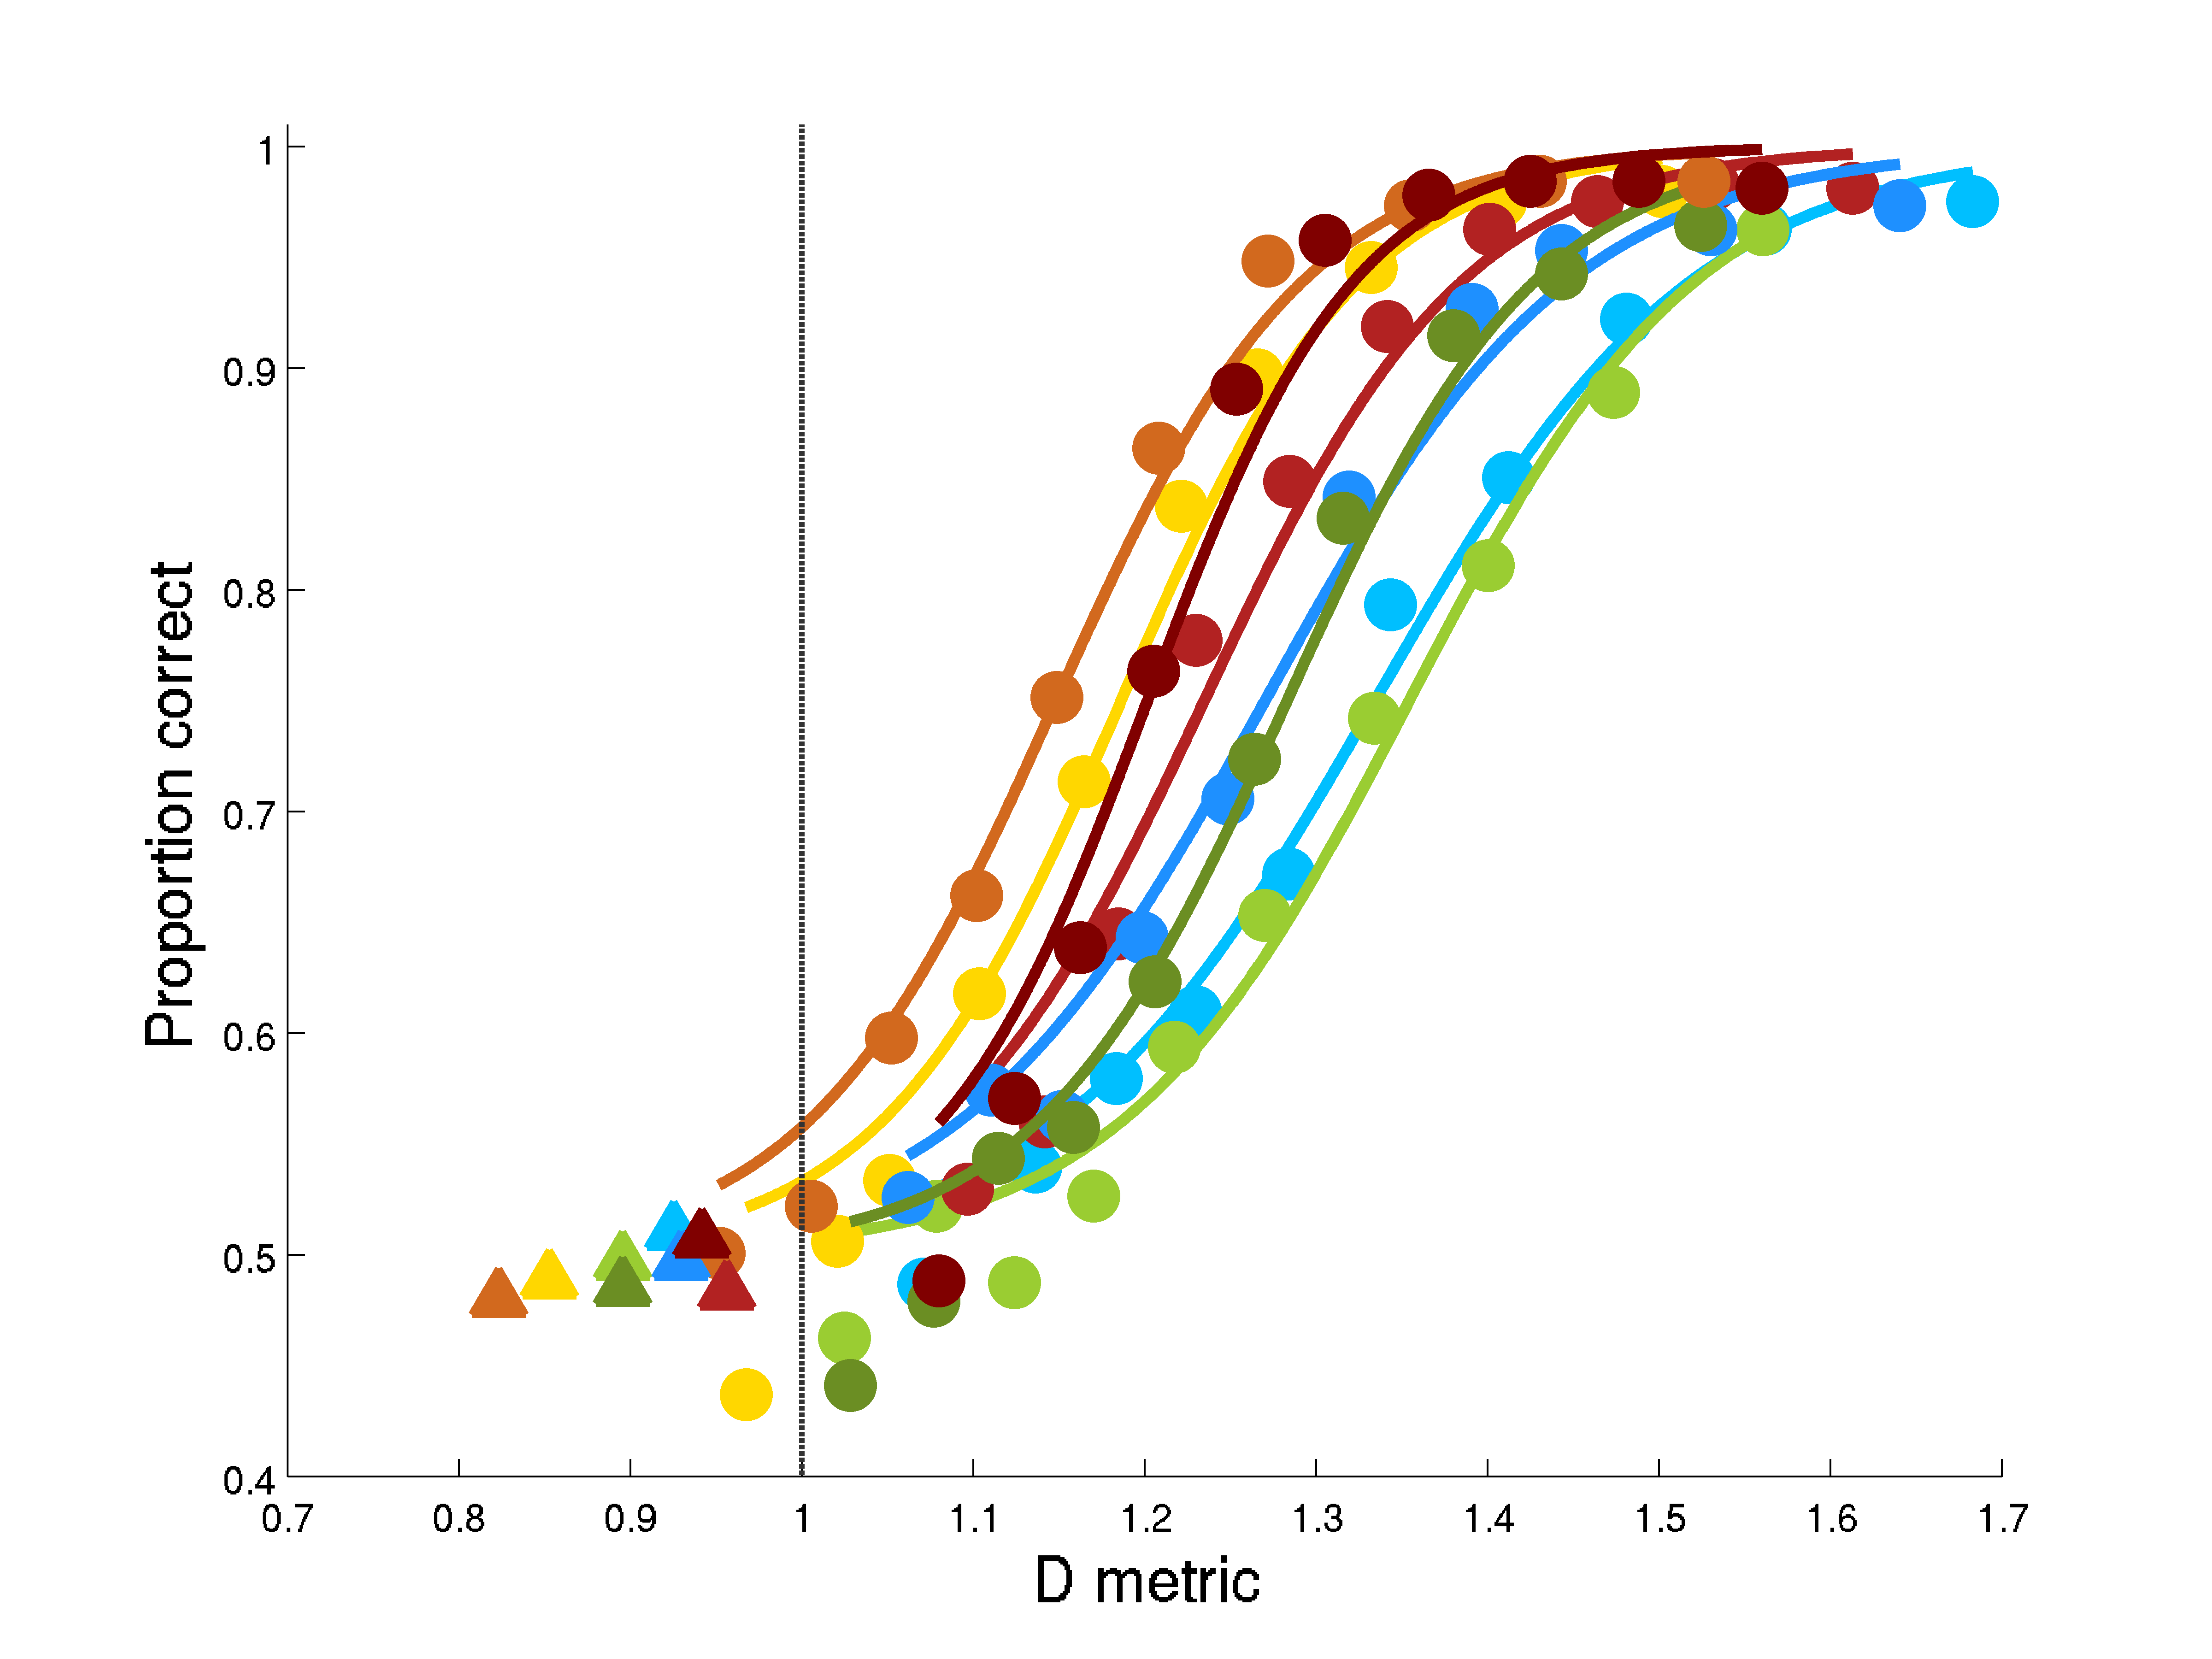
\includegraphics{Figures/FIG_SUP_D.png}
\caption{Dependence of human performance on D for Experiment 1 (circles) and Experiment 2 (triangles). The curve fits are performed only on the data points of Experiment 1. Color code as in the manuscript.}
\label{fig_D}
\end{figure}



%%
% Luminance
%%
\section{Comparison with a luminance metric}

As noted in the Introduction to the main text, contour detection in pathfinder displays can be achieved not only through explicit grouping mechanisms, but also via the application of a low-pass luminance filter to the input. Such image smoothing could result in the physical linking of the luminance values around closer element pairings, thereby providing a direct cue to the location of the contour.\\

Here we investigate the performance of a metric based on low-pass filtered versions of our stimuli. We should note that such a metric suffers from a similar problem as D (\autoref{section_comparison_D}): It yields only a single, global value per display, which does not allow the analyses performed in the manuscript. We here compute the average luminance after smoothing, separately for pixels in a narrow region (minimum distance between background elements) around the contour and for pixels in the background region. The average luminance difference between the contour and background regions then serves as the density metric. The smoothing was done by applying Gaussian low-pass filters in the frequency domain, centered on the DC component. The correspondence between this luminance metric and human performance is plotted in \autoref{fig_luminance} for two different widths of the Gaussian frequency filter (15 and 25 cycles per image). It can be seen that the filter width has little impact, and that the luminance metric has a much weaker relation to human performance for the open contours, compared to the closed contours. But even for the latter, the average performance is around 65\% correct when the cue should have been eliminated (luminance difference equals zero). This is considerably worse than the best-performing metrics in the manuscript.\\

\begin{figure}
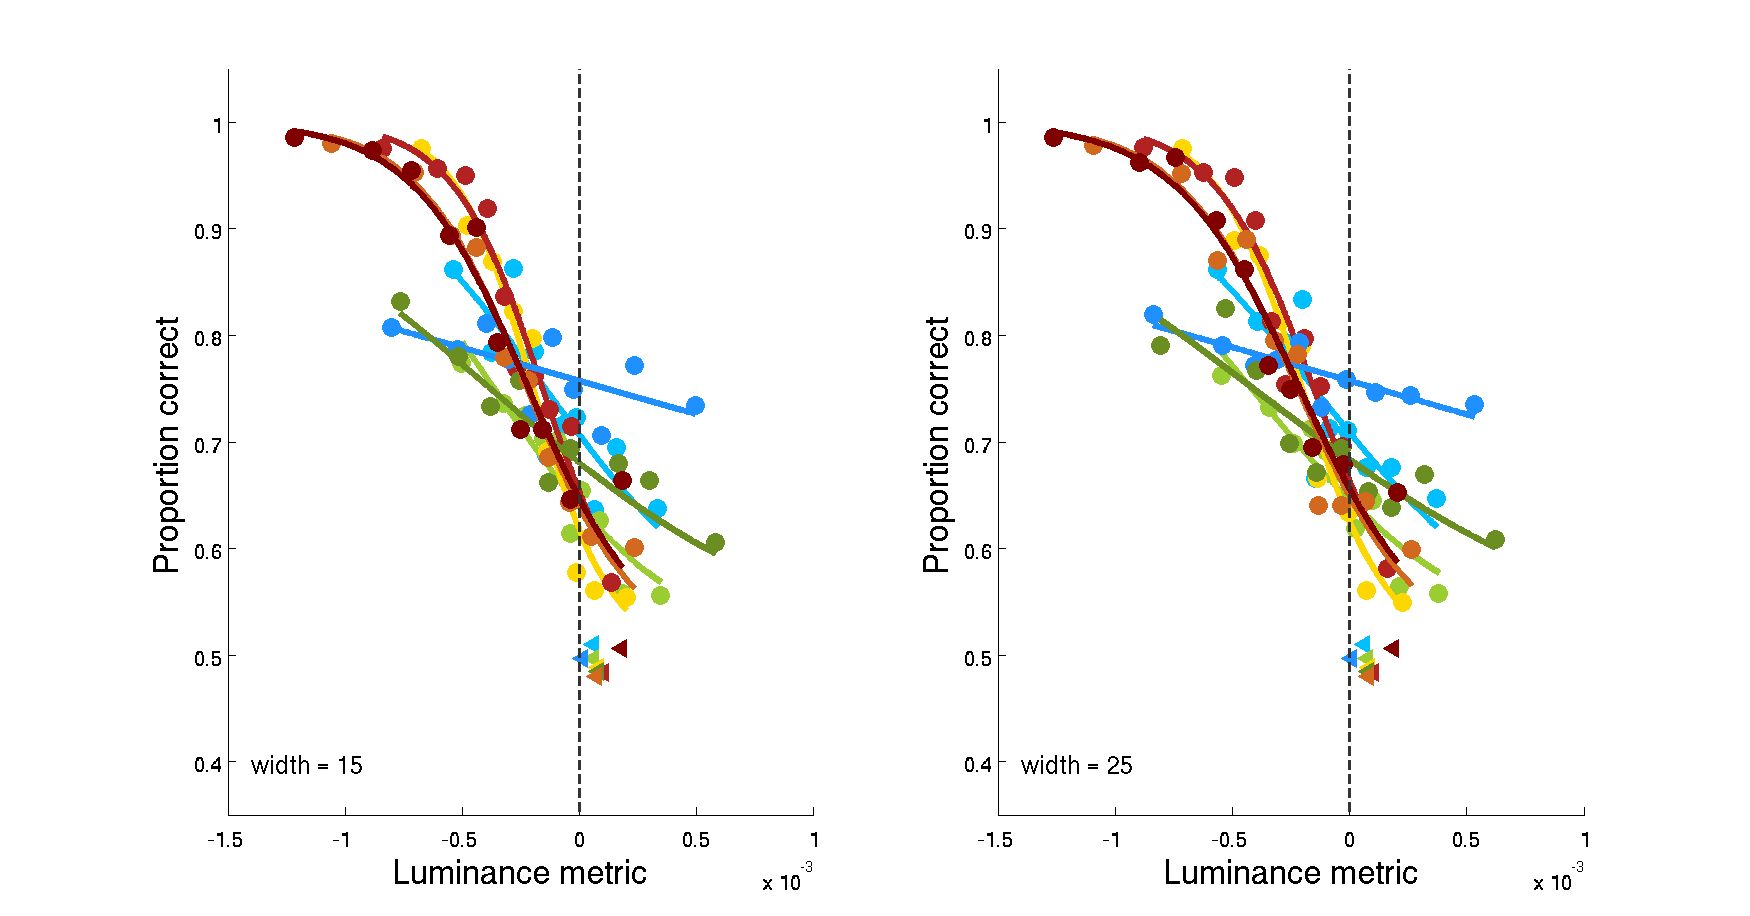
\includegraphics{Figures/FIG_SUP_luminance.png}
\caption{Relation between the luminance difference between contour and background elements in low-pass filtered versions of the stimuli, and the average proportion correct across all participants in Experiment 1 (circles) and Experiment 2 (triangles). The curve fits are performed only on the data points of Experiment 1. Color code as in the manuscript. The panels represent different filter widths.}
\label{fig_luminance}
\end{figure}



%%
% References
%%

\bibliography{supplement.bib}{}
\bibliographystyle{apacite}


%%
% The End
%%
\end{document}